% Tài liệu kỹ thuật (tiếng Việt).
% Biên dịch:  cd reports/technical_document && latexmk -pdf report_vi.tex     (hoặc: xelatex/pdflatex report_vi.tex, chạy 2 lần)
% Hình do ../make_figures.py sinh ra từ nhật ký chạy thật trong docs/data/.
\documentclass[11pt,a4paper]{article}

\usepackage{iftex}
\ifPDFTeX
  \usepackage[utf8]{inputenc}
  \usepackage[T5]{fontenc}
  \usepackage{lmodern}
\else
  \usepackage{fontspec}
\fi
\usepackage[margin=2.5cm]{geometry}
\usepackage{amsmath,amssymb}
\usepackage{graphicx}
\usepackage{booktabs}
\usepackage{array}
\usepackage{float}
\usepackage{caption}
\usepackage[hidelinks]{hyperref}
\usepackage{url}

\graphicspath{{../figures/}{../../docs/}}
\renewcommand{\figurename}{Hình}
\renewcommand{\tablename}{Bảng}
\renewcommand{\contentsname}{Mục lục}
\renewcommand{\arraystretch}{1.15}
\captionsetup{font=small,labelfont=bf}
\setlength{\parskip}{4pt}
\setlength{\parindent}{0pt}
\emergencystretch=3em
\newcommand{\code}[1]{\texttt{\small #1}}

\title{\textbf{Tài liệu kỹ thuật và thiết kế hệ thống}\\[4pt]
\large Robot di động đa hướng 4 bánh điều khiển bằng cử chỉ hai bàn tay\\
\normalsize Dự án AI-Powered Omni Robot, phiên bản 2}
\author{Tai Nguyen Anh}
\date{Tháng 11 năm 2026}

\begin{document}
\maketitle
\tableofcontents
\newpage

%====================================================================
\section{Tổng quan hệ thống}
\subsection{Bài toán và mục tiêu}
Robot dẫn động vi sai không trượt ngang được, còn robot omni bố trí 4 bánh chéo $45^\circ$ chuyển động theo mọi hướng trên mặt phẳng với ba vận tốc độc lập: tiến ($v_x$), ngang ($v_y$) và xoay ($\omega$). Giao diện điều khiển cử chỉ thường chỉ lo việc lái, còn đổi chế độ, chỉnh tốc độ hay bấm dừng khẩn cấp vẫn cần chuột hoặc bàn phím.

Dự án làm hai việc cùng lúc, chỉ với một camera laptop:
\begin{itemize}
  \item \textbf{Tay thuận} điều khiển giao diện web: di con trỏ, giữ yên để click, duỗi ngón giữa để bấm hoặc kéo cần lái và thanh trượt.
  \item \textbf{Tay không thuận} lái robot bằng 8 hướng chỉ tay và chữ V để xoay. Ở chế độ Thủ công (cần lái ảo, bàn phím) chỉ cần một tay bất kỳ để điều khiển giao diện.
\end{itemize}
Phần cứng thực thi là robot dùng ESP32, hai mạch cầu H L298N và bốn động cơ GM25-370 có encoder. ESP32 tự phát Wi-Fi và nhận lệnh qua UDP.

\subsection{Chỉ tiêu và kết quả đo}
Các chỉ tiêu trong Bảng~\ref{tab:spec} do nhóm tự đặt làm mốc tham chiếu, không phải yêu cầu từ bên ngoài. Cột kết quả lấy từ các lần đo trong mục~\ref{sec:verify}.

\begin{table}[H]
\caption{Chỉ tiêu đặt ra và kết quả đo được.}
\label{tab:spec}
\centering\small
\begin{tabular}{p{4.6cm}p{2.3cm}p{5.2cm}}
\toprule
Hạng mục & Chỉ tiêu & Kết quả đo \\
\midrule
Tốc độ vòng camera + nhận diện tay & $\ge 25$ fps & 29,9 fps; suy luận trung bình 18,5 ms (P95 27,1 ms), khi chưa có tay trong khung \\
Độ trễ khứ hồi UDP (RTT) & $<50$ ms (trung vị) & trung vị 6,6--8,1 ms; P95 16,1--26,1 ms \\
Sai số bám tốc độ từng bánh (trung bình) & $<5{,}0\,\%$ & 1,5--3,2\,\% tốc độ tối đa; P95 4,4--7,4\,\% \\
Sai lệch vận tốc thân robot so với lệnh & $<5{,}0\,\%$ & 0,1--2,5\,\% theo trục chính; trục khác $\le 0{,}004$ \\
Từ lúc chốt cử chỉ đến khi bánh đạt 50\,\% & $<400$ ms & trung vị 257--260 ms (203--359 ms) \\
Ngắt an toàn khi mất lệnh & $<500$ ms & ESP32 300 ms; laptop 400 ms; chống kẹt bánh 700 ms \\
\bottomrule
\end{tabular}
\end{table}
Chú ý: tốc độ 29,9 fps và suy luận 18,5 ms đo ngày 12/11/2026 trên 359 khung liên tiếp; độ trễ cử chỉ đến bánh đã gồm giới hạn gia tốc có chủ ý (mục~\ref{sec:control}) và chưa gồm 4 khung (khoảng 133 ms) cần để chốt cử chỉ.

\subsection{Kiến trúc tổng thể}
Hệ thống gồm hai phân hệ nối với nhau bằng Wi-Fi do chính ESP32 phát (SSID \code{omni-robot}, IP cố định \code{192.168.4.1}, cổng UDP 4210), không cần Internet (Hình~\ref{fig:arch}).

\begin{itemize}
  \item \textbf{Laptop (host)}: \code{ai/camera.py} đọc ảnh MJPG $640\times480$ ở 30 fps trong một luồng riêng, chỉ giữ khung mới nhất. MediaPipe HandLandmarker lấy 21 điểm mốc cho tối đa 2 tay. \code{RoleAssigner} và \code{split\_roles()} chia tay thuận (con trỏ, \code{ai/ui/cursor.py}) và tay không thuận (cử chỉ lái, \code{ai/drive/}). Vòng \code{control\_loop()} 20 Hz chọn lệnh theo chế độ, giới hạn gia tốc rồi gửi UDP qua \code{RobotLink}.
  \item \textbf{ESP32 (edge)}: nhận gói lệnh, kiểm tra quyền chủ duy nhất và hạn 300 ms, tính động học nghịch, chạy 4 bộ điều khiển tốc độ mỗi 10 ms, xuất PWM ra hai L298N và trả về gói phản hồi gồm tốc độ đặt, tốc độ đo và PWM của 4 bánh.
\end{itemize}

\begin{figure}[H]
  \centering
  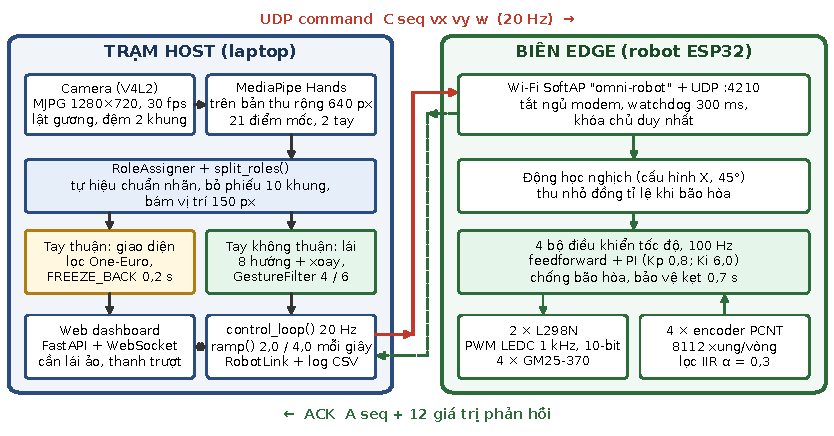
\includegraphics[width=\textwidth]{fig_arch_vi.pdf}
  \caption{Kiến trúc host--edge. Đường đỏ liền: lệnh UDP; đường xanh đứt: phản hồi kèm số liệu 4 bánh.}
  \label{fig:arch}
\end{figure}

%====================================================================
\section{Cơ khí và động học}
\subsection{Cấu hình}
Bốn bánh omni đặt ở bốn góc, trục lăn chính nghiêng $\pm45^\circ$ so với trục dọc thân (kiểu chữ X), gắn trực tiếp vào trục ra của bốn động cơ giảm tốc $1{:}78$. Mã dùng quy ước ROS: $+x$ về phía trước, $+y$ sang trái, $+\omega$ ngược chiều kim đồng hồ khi nhìn từ trên (Hình~\ref{fig:kin}). Chỉ số bánh: 0 trước trái (tt), 1 trước phải (tp), 2 sau trái (st), 3 sau phải (sp). Tốc độ bánh dương là chiều làm robot tiến.

\begin{figure}[H]
  \centering
  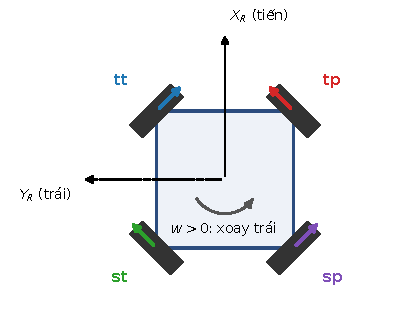
\includegraphics[width=0.5\textwidth]{fig_kin_vi.pdf}
  \caption{Hình học cấu hình X và hướng đẩy của từng bánh khi quay tiến.}
  \label{fig:kin}
\end{figure}

\subsection{Động học nghịch và bảo toàn hướng}
Trong firmware (\code{firmware/src/kinematics.h}) vận tốc được chuẩn hóa vào $[-1,1]$, mức 1,0 ứng với \code{MAX\_CPS} $=4300$ xung/giây (khoảng 31,8 vòng/phút). Với $\mathbf u=[v_x,v_y,\omega]^\top$:
\begin{equation}
\begin{bmatrix}r'_{tt}\\r'_{tp}\\r'_{st}\\r'_{sp}\end{bmatrix}=
\begin{bmatrix}1&-1&-1\\1&1&1\\1&1&-1\\1&-1&1\end{bmatrix}\mathbf u,\qquad
r_i=\frac{r'_i}{m},\quad m=\max\bigl(1,\max_j|r'_j|\bigr).
\label{eq:ik}
\end{equation}
Chia chung cho $m$ giữ nguyên tỉ lệ giữa các bánh khi có bánh vượt 1,0, nên robot chỉ chậm lại chứ không đổi hướng. Nếu cắt từng bánh riêng, tỉ lệ bị méo và robot đi lệch.

\subsection{Động học thuận}
Các cột của ma trận trong (\ref{eq:ik}) trực giao và có bình phương độ dài bằng 4, nên nghịch đảo giả là ma trận chuyển vị chia 4. Từ tốc độ đo $m_i$ của 4 bánh, \code{tests/analyze\_drive\_log.py} tính lại vận tốc thân:
\begin{equation}
\begin{bmatrix}v_x\\v_y\\\omega\end{bmatrix}_{\text{đo}}=\frac14
\begin{bmatrix}1&1&1&1\\-1&1&1&-1\\-1&1&-1&1\end{bmatrix}
\begin{bmatrix}m_{tt}\\m_{tp}\\m_{st}\\m_{sp}\end{bmatrix}.
\label{eq:fk}
\end{equation}

%====================================================================
\section{Phần cứng và điện}
\subsection{Nguồn và mạch công suất}
Nguồn chính 12 V nuôi hai L298N và bốn động cơ. L298N dùng transistor lưỡng cực nên sụt áp nội bộ lớn, cỡ 1,5--2 V theo đặc tính chung của loại IC này (chưa đo riêng trên mạch), vì vậy chọn 12 V. Tốc độ tối đa đo được của bốn bánh là 4552--4869 xung/giây (33,7--36,0 vòng/phút); \code{MAX\_CPS} lấy 4300, thấp hơn bánh chậm nhất để bộ điều khiển còn dư PWM mà bù. PWM dùng ngoại vi LEDC của ESP32 ở 1 kHz, 10 bit, vì thời gian đóng cắt của L298N chậm.

Encoder cấp 3,3 V cho khớp mức logic với ESP32, ngõ ra kiểu đẩy-kéo nên điện trở kéo nội bị tắt trong phần mềm, và bốn encoder dùng chung dây GND với ESP32.

\subsection{Quy hoạch chân GPIO}
Có 20 chân tín hiệu: 4 PWM, 8 chân chiều (IN1, IN2) và 8 chân encoder (pha A, B). Các chân chỉ-vào của ESP32 (GPIO 34, 35, 36, 39) dùng cho encoder hai bánh trước, nhường chân xuất cho L298N (Bảng~\ref{tab:pins}, sơ đồ ở Hình~\ref{fig:pinout}).

\begin{table}[H]
\caption{Chân GPIO (\code{firmware/src/robot\_config.h}).}
\label{tab:pins}
\centering\small
\begin{tabular}{lccccc}
\toprule
Bánh & PWM & IN1 & IN2 & Encoder A & Encoder B \\
\midrule
0 trước trái (tt) & 25 & 26 & 27 & 36 & 39 \\
1 trước phải (tp) & 13 & 23 & 22 & 34 & 35 \\
2 sau trái (st)   & 21 & 19 & 18 & 32 & 33 \\
3 sau phải (sp)   & 17 & 16 & 4  & 14 & 5  \\
\bottomrule
\end{tabular}
\end{table}
Hai động cơ bên phải lắp đối xứng gương nên encoder đếm ngược dấu: \code{ENCODER\_INVERT} $=\{$false, true, false, true$\}$. Động cơ sau phải đấu dây ngược chiều, được bù bằng \code{MOTOR\_INVERT} $=\{$false, false, false, true$\}$. Nhờ vậy ở mọi chỗ khác trong mã, PWM dương luôn làm bánh quay tiến và tốc độ đo luôn dương khi tiến.

\begin{figure}[H]
  \centering
  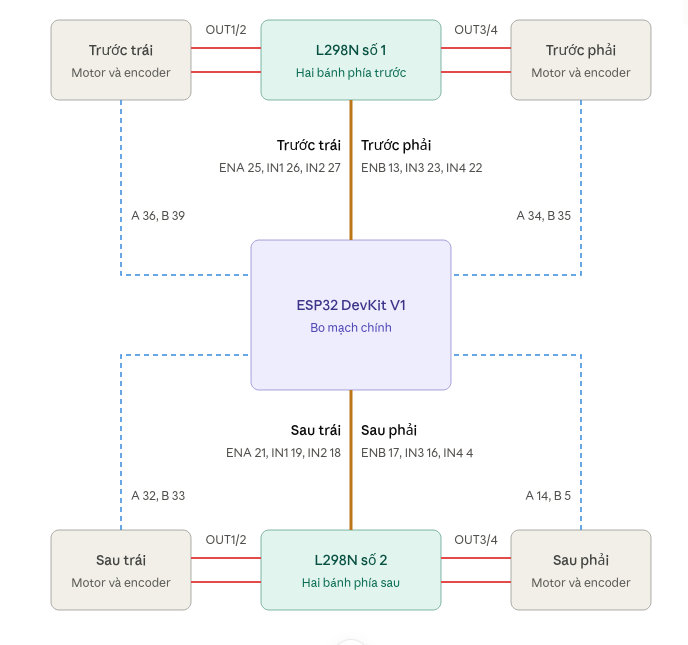
\includegraphics[width=0.85\textwidth]{pinout.png}
  \caption{Sơ đồ đấu nối ESP32 DevKit V1, hai L298N và bốn động cơ GM25-370 có encoder (\code{docs/pinout.png}).}
  \label{fig:pinout}
\end{figure}

%====================================================================
\section{Phần mềm}
\subsection{Nhận diện hai bàn tay}
Nhận diện dùng hình học trên 21 điểm mốc của MediaPipe (chế độ VIDEO, ngưỡng tin cậy 0,6), không huấn luyện thêm.

\textbf{Ngón duỗi.} Một ngón duỗi khi khoảng cách từ đầu ngón đến cổ tay lớn hơn 1,15 lần khoảng cách từ khớp giữa (PIP) đến cổ tay. Tỉ số không có đơn vị nên không phụ thuộc khoảng cách tới camera hay góc xoay của bàn tay. Chỉ ngón trỏ duỗi thì hướng chỉ được tính từ gốc ngón (điểm 5) đến đầu ngón (điểm 8) và chia 8 múi $45^\circ$.

\textbf{Phân vai.} Ảnh đã lật gương nhưng MediaPipe gán nhãn Left/Right như thể chưa lật, nên nhãn bị ngược từ góc nhìn người dùng. \code{RoleAssigner} xử lý như sau:
\begin{enumerate}
  \item Hai tay: vai theo thứ tự hoành độ cổ tay; sai lệch giữa thứ tự này và nhãn (đã đảo) cập nhật điểm $c_k=0{,}95\,c_{k-1}\pm0{,}05$, khi $c_k<-0{,}6$ thì đảo quy ước nhãn.
  \item Một tay: bỏ phiếu nhãn trong 10 khung gần nhất.
  \item Vừa từ hai tay còn một tay và cổ tay dịch dưới 150 px: giữ vai cũ.
  \item Chế độ Thủ công (\code{drive\_active = False}): nhánh lái bị khóa, bất kỳ tay nào cũng là tay giao diện.
\end{enumerate}

\textbf{Lọc cử chỉ lái.} \code{GestureFilter} cần 4 khung liên tiếp (khoảng 0,13 s) để bắt đầu một lệnh chuyển động và 6 khung (khoảng 0,2 s) để dừng, nên một khung nhiễu thoáng qua không làm robot giật.

\subsection{Con trỏ giao diện}
Tay thuận có ba tư thế: \emph{point} (chỉ ngón trỏ) di con trỏ, \emph{click} (trỏ cộng giữa) để bấm hoặc kéo, \emph{idle} (khác) ẩn con trỏ để tránh bấm nhầm. Một tư thế phải giữ 3 khung mới được chấp nhận; mất tay quá 0,3 s thì con trỏ ẩn và mọi nút đang giữ được nhả.

Vị trí đầu ngón trỏ được làm mượt bằng bộ lọc One-Euro ($f_{\min}=1$ Hz, $\beta=8$ trên toạ độ chuẩn hóa), tần số cắt $f_c=f_{\min}+\beta|\dot x|$ thấp khi tay yên và tăng theo tốc độ tay.

\textbf{Neo điểm tác động (\code{FREEZE\_BACK}).} Duỗi thêm ngón giữa để click có thể kéo đầu ngón trỏ lệch khỏi nút đang nhắm (đo thật ở mục~\ref{sec:verify}). Khi tư thế đổi từ point sang click tại thời điểm $t$, hệ thống lấy vị trí đã lọc gần nhất cách đó ít nhất 0,2 s làm gốc và giữ độ lệch bù suốt lúc click:
\begin{equation}
(x_a,y_a)=(x_j,y_j),\ j=\arg\max\{t_j:\ t-t_j\ge0{,}2\},\qquad
(a_x,a_y)=\mathrm{clamp}\bigl(x+x_a-x(t),\ y+y_a-y(t)\bigr).
\end{equation}
Con trỏ hiển thị vẫn bám đầu ngón tay nên kéo vẫn mượt. Sau khi nhả, độ lệch giảm theo hàm mũ với hằng số thời gian 0,15 s (\code{OFFSET\_TAU}). Thanh trượt dùng nắm tương đối: giữ yên để nắm, di ngón tay để kéo, giữ yên lần nữa để nhả. Hình~\ref{fig:click} minh họa trên bàn tay mô phỏng.

\begin{figure}[H]
  \centering
  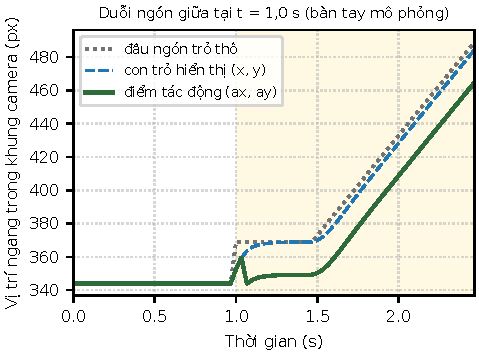
\includegraphics[width=0.6\textwidth]{fig_click_vi.pdf}
  \caption{Neo điểm tác động trên bàn tay mô phỏng (dùng chính lớp \code{Cursor}). Duỗi ngón giữa tại $t=1{,}0$ s làm đầu ngón dịch 25 px.}
  \label{fig:click}
\end{figure}

\subsection{Giao thức truyền thông}
Lệnh chuyển động liên tục 20 Hz chỉ có giá trị mới nhất là hữu ích, nên chọn UDP: gói rớt bị bỏ qua và 50 ms sau có gói thay thế, còn TCP sẽ giữ các gói mới sau gói bị mất. Trên ESP32 tắt chế độ ngủ của modem Wi-Fi (\code{WiFi.setSleep(false)}) để giảm trễ. Khung truyền là văn bản ASCII, dễ gỡ lỗi:
\begin{center}\small
\code{C <seq> <vx> <vy> <w>}\quad (laptop $\to$ ESP32), ví dụ \code{C 142 0.500 -0.200 0.000}\\
\code{A <seq> <m0 d0 p0 ... m3 d3 p3>}\quad (ESP32 $\to$ laptop; muốn, đo, PWM của 4 bánh)
\end{center}
\textbf{An toàn nhiều tầng.} (1) ESP32 chỉ nhận lệnh từ máy gửi hợp lệ đầu tiên và từ chối địa chỉ khác cho đến khi máy đó im quá 300 ms. (2) ESP32 trả lệnh $(0,0,0)$ nếu quá 300 ms không có gói mới. (3) Laptop đặt vận tốc đích về 0 nếu quá 0,4 s không có lệnh mới từ chế độ đang chọn. (4) Bộ giới hạn \code{ramp()} có gia tốc tối đa 2,0/giây, giảm tốc tối đa 4,0/giây, và bắt buộc đi qua 0 trước khi đổi dấu vận tốc.

\subsection{Điều khiển vòng kín trên ESP32}\label{sec:control}
Mỗi chu kỳ 10 ms (100 Hz), \code{firmware/src/wheel.h} đọc số xung từ bộ đếm phần cứng PCNT ở chế độ giải mã vuông pha $\times4$ (8112 xung/vòng bánh = 26 xung/kênh $\times4\times78$) kèm bộ lọc nhiễu phần cứng 12,5 $\mu$s, nên việc đếm xung không tốn thời gian CPU. Vì một xung trong 10 ms đã bằng 2,3\,\% tốc độ tối đa, tốc độ đo được lọc thông thấp bậc 1:
\begin{equation}
\omega_i(k)=0{,}7\,\omega_i(k-1)+0{,}3\,\frac{c_i(k)}{4300},
\end{equation}
với $c_i$ là số xung trên giây. Mục tiêu $r_i$ của mỗi bánh tiến dần đến giá trị đặt với độ dốc tối đa 4,0/giây. Luật điều khiển (Hình~\ref{fig:ctrl}):
\begin{align}
u^{\mathrm{ff}}_i&=\operatorname{sgn}(r_i)\bigl(a_i+b_i|r_i|\bigr), \quad e_i=r_i-\omega_i,\\
I_i&\leftarrow I_i+K_i e_i\,\Delta t\quad\text{chỉ khi không đang tăng tốc và chưa bão hòa},\\
u_i&=\mathrm{clamp}\bigl(u^{\mathrm{ff}}_i+K_p e_i+I_i,\,-1,\,1\bigr),\qquad K_p=0{,}8,\ K_i=6{,}0.
\end{align}
Hệ L298N cộng GM25-370 rất phi tuyến: ngưỡng PWM để bánh bắt đầu quay khác nhau giữa các bánh (5,5\,\% đến 14,8\,\%, gấp 2,7 lần) và khoảng 44\,\% PWM đã cho 80\,\% tốc độ không tải. Các hệ số $a_i$, $b_i$ (Bảng~\ref{tab:ff}) là đường thẳng khớp bình phương tối thiểu từ các điểm xác lập đo khi kê bánh lơ lửng, bằng công cụ \code{firmware/tools/motor\_test.cpp}; độ lệch khớp tối đa 0,045 PWM. Khâu feedforward đưa PWM gần đúng ngay, khâu PI chỉ phải bù phần còn lại (đặc biệt là tải thật trên sàn). Đóng băng tích phân khi đang tăng tốc hoặc bão hòa nhằm tránh tích lũy sai số trong lúc mục tiêu còn chạy (windup). Chưa có phép so sánh với PID thuần hay vòng hở trên cùng quỹ đạo nên chưa định lượng được mức cải thiện.

\textbf{Bảo vệ kẹt.} Nếu PWM từ 0,95 trở lên mà tốc độ đo dưới 0,05 liên tục quá 0,7 s (\code{STALL\_SECONDS}), bánh đó bị ngắt và báo lỗi qua Serial cho đến khi lệnh về 0.

\begin{figure}[H]
  \centering
  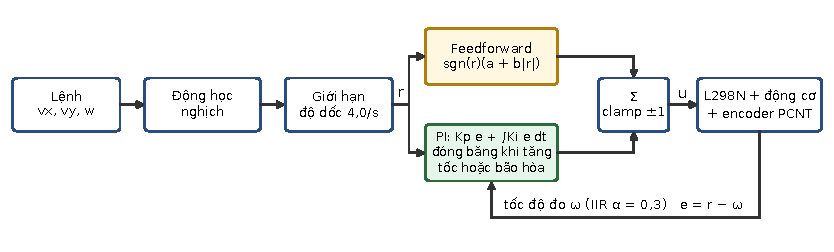
\includegraphics[width=\textwidth]{fig_ctrl_vi.pdf}
  \caption{Bộ điều khiển tốc độ của một bánh (chu kỳ 100 Hz).}
  \label{fig:ctrl}
\end{figure}

\begin{table}[H]
\caption{Tham số feedforward đo được và sai số bám trung bình trên sàn (\% tốc độ tối đa).}
\label{tab:ff}
\centering\small
\begin{tabular}{lccccc}
\toprule
Bánh & $a_i$ (\code{FF\_OFFSET}) & $b_i$ (\code{FF\_SLOPE}) & Thủ công v1 & Cử chỉ v1 & Hai tay v2 \\
\midrule
tt & 0,076 & 0,470 & 1,8 & 1,9 & 2,5 \\
tp & 0,148 & 0,594 & 3,2 & 2,5 & 2,6 \\
st & 0,055 & 0,453 & 1,7 & 1,6 & 2,3 \\
sp & 0,060 & 0,464 & 1,5 & 1,7 & 2,5 \\
\bottomrule
\end{tabular}
\end{table}

\subsection{Giao diện web}
Dashboard (FastAPI, WebSocket, một trang không cuộn) có hai chế độ: Thủ công (cần lái ảo, nút xoay, phím mũi tên hoặc W A S D, Q E, Space) và Cử chỉ tay. Mọi nút, thanh trượt và cần lái đều thao tác được bằng con trỏ tay thuận; ánh xạ cử chỉ ở Bảng~\ref{tab:gest}. Hình~\ref{fig:ui} chụp từ bản chạy thật, không gắn camera.
\begin{figure}[H]
  \centering
  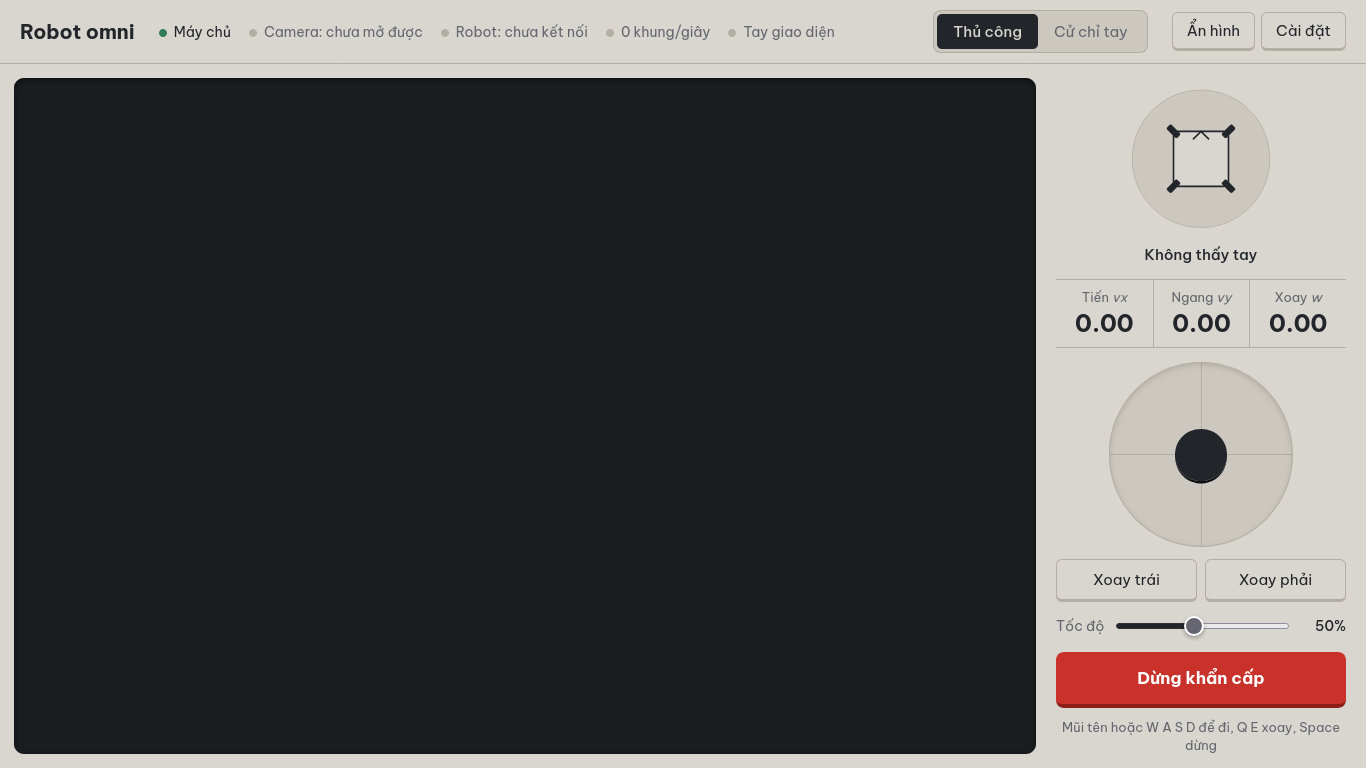
\includegraphics[width=0.9\textwidth]{dashboard.png}
  \caption{Dashboard ở chế độ Thủ công.}
  \label{fig:ui}
\end{figure}

\begin{table}[H]
\caption{Ánh xạ cử chỉ ($s\in[0{,}1;1]$ là hệ số tốc độ).}
\label{tab:gest}
\centering\small
\begin{tabular}{p{2.4cm}p{3.6cm}p{5.6cm}}
\toprule
Tay & Cử chỉ & Tác dụng \\
\midrule
Không thuận & nắm, xòe, mất tay & Dừng: $(0,0,0)$ \\
Không thuận & trỏ lên / xuống & Tiến $(+s,0,0)$ / lùi $(-s,0,0)$ \\
Không thuận & trỏ trái / phải & Sang trái $(0,+s,0)$ / phải $(0,-s,0)$ \\
Không thuận & trỏ chéo & Đi chéo $(\pm0{,}707s,\pm0{,}707s,0)$ \\
Không thuận & chữ V trái / phải & Xoay trái $(0,0,+s)$ / phải $(0,0,-s)$ \\
Thuận & trỏ & Di con trỏ; giữ yên 0,8 s để click hoặc nắm thanh trượt \\
Thuận & trỏ cộng giữa & Click nhanh; giữ và di để kéo \\
Thuận & khác, mất tay & Ẩn con trỏ, nhả mọi nút giữ \\
\bottomrule
\end{tabular}
\end{table}

%====================================================================
\section{Kiểm thử và phân tích số liệu}\label{sec:verify}
\subsection{Kiểm thử tự động}
\begin{itemize}
  \item \code{tests/test\_hands\_logic.py}: 46 kiểm tra trên bàn tay giả dựng bằng toán, gồm phân loại cử chỉ, tư thế giao diện, phân vai khi nhãn bị ngược, tự hiệu chuẩn, bộ lọc One-Euro, neo điểm tác động. Kết quả: 46/46 đạt.
  \item \code{tests/handcursor\_test.html}: 49 kiểm tra trong trình duyệt cho dwell click, click hai ngón, nắm tương đối thanh trượt, kéo cần lái, nút giữ, tự nhả khi mất tay, thẻ thông số. Chạy bằng Chrome không giao diện (cửa sổ $1280\times900$) ngày 12/11/2026: 49/49 đạt. Cửa sổ quá thấp (dưới khoảng 500 px) làm một kiểm tra vị trí con trỏ báo lỗi giả vì con trỏ bị kẹp vào mép cửa sổ.
\end{itemize}
Các kiểm tra tự động dùng bàn tay mô phỏng, nên con số của chúng chỉ mô tả thuật toán trên dữ liệu lý tưởng. Với nhiễu 2 px (200 lần chạy có hạt giống) độ lệch chuẩn của con trỏ giảm từ 0,0047 xuống 0,0016 (giảm 65,5\,\%). Với ngón trỏ bị lệch $(25,-15)$ px khi duỗi ngón giữa, điểm tác động lệch 0,0126 (đơn vị chuẩn hóa) so với 0,0770 của đầu ngón, giảm 83,6\,\%; phần dư là 4,6 px trong 29,2 px. Vì tư thế click chỉ được chấp nhận sau 3 khung, điểm tác động có thể lệch thoáng qua tới 15,6 px (khoảng 0,1 s) trước khi bù.

\textbf{Đo trên bàn tay thật.} Chạy \code{tests/real\_hand\_eval.py} (cùng lớp \code{Cursor}, ảnh camera thật, một người thử), dữ liệu \code{docs/data/v2/real\_hand\_click\_still.csv} và \code{real\_hand\_jitter.json}. \emph{Rung khi giữ yên:} giữ yên ngón trỏ 8 giây (209 khung), độ lệch chuẩn của đầu ngón thô là 2,26 px và của con trỏ sau lọc là 2,14 px, chỉ giảm 5\,\% (mô phỏng cho 65,5\,\%). Mô phỏng dùng nhiễu độc lập, còn rung và trôi điểm mốc thật nhiều khả năng chậm và có tương quan nên bộ lọc thông thấp đang chỉnh cho nhạy không loại bỏ được; chưa kiểm tra giả thuyết này. \emph{Lệch khi click:} người thử chỉ ngón trỏ vào một điểm và giữ yên (script chờ đầu ngón nằm trong 3 px suốt 1 giây và loại lần nào tay còn trôi), rồi duỗi ngón giữa, 12 lần. Đầu ngón trỏ dịch trung vị 1,65 px (1,1--5,7), nhỏ hơn rất nhiều so với 29,2 px giả định trong mô phỏng. Điểm tác động có neo dịch trung vị 4,15 px (2,0--12,0), nhiều hơn đầu ngón ở 11 trong 12 lần (Hình~\ref{fig:real}); con trỏ hiển thị dịch 1,9 px. Như vậy với người thử này, khi giữ yên ngón tay, độ lùi 0,2 s làm thêm khoảng 2,5 px thay vì bù độ lệch. Nguyên nhân có thể là độ dịch thật cùng cỡ với rung tay nên neo lấy mẫu đúng phần rung thay vì sửa một cú giật có hệ thống. Một lần đo trước đó không giữ yên ngón tay cho độ dịch trung vị 6,8 px và không được dùng. Đây là 12 lần của một người; chưa đo tỉ lệ bấm trúng, và bán kính dwell (30 px) cùng kích thước nút đều lớn hơn các độ lệch này nên tác động thực tế lên việc bấm nhiều khả năng nhỏ nhưng chưa kiểm chứng. Với người dùng hoặc dáng tay khác mà ngón trỏ giật mạnh hơn, neo vẫn có thể có ích.

\begin{figure}[H]
  \centering
  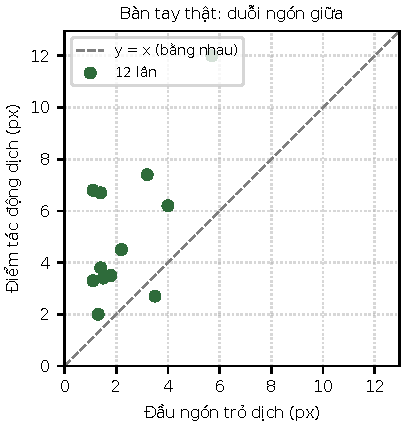
\includegraphics[width=0.45\textwidth]{fig_real_vi.pdf}
  \caption{Bàn tay thật, 12 lần giữ yên ngón tay: độ dịch của điểm tác động so với đầu ngón trỏ thô khi duỗi ngón giữa. Điểm trên đường đứt là điểm tác động dịch nhiều hơn đầu ngón.}
  \label{fig:real}
\end{figure}

\subsection{Số liệu chạy thật}
Ba phiên chạy trên sàn nhà, ghi 20 Hz, được phân tích bằng \code{tests/analyze\_drive\_log.py}; dữ liệu ở \code{docs/data/v1/} và \code{docs/data/v2/} (Bảng~\ref{tab:data}). Các dòng ghi lúc nguồn motor tắt (53 dòng ở phiên thủ công) được loại bỏ.

\begin{table}[H]
\caption{Các phiên chạy.}
\label{tab:data}
\centering\small
\begin{tabular}{>{\raggedright\arraybackslash}p{5.2cm}rr>{\raggedleft\arraybackslash}p{3.4cm}}
\toprule
Phiên (tệp) & Dòng & Thời lượng (s) & RTT trung vị / P95 / lớn nhất (ms) \\
\midrule
Thủ công v1 (\code{drive\_manual.csv}) & 3240 & 1512 & 7,8 / 22,5 / 97 \\
Cử chỉ v1 (\code{drive\_gesture.csv}) & 4820 & 247 & 8,1 / 26,1 / 101 \\
Hai tay v2 (\code{drive\_twohand.csv}) & 5020 & 266 & 6,6 / 16,1 / 909 \\
\midrule
Tổng & 13080 & 2026 & -- \\
\bottomrule
\end{tabular}
\end{table}
Trong phiên thủ công có 389 dòng ở chế độ cử chỉ. RTT lớn nhất ở phiên v2 là 909 ms, vượt xa hạn 300 ms của ESP32 nên robot sẽ dừng trong trường hợp đó.

\textbf{Độ trễ.} Từ lúc cử chỉ di chuyển được ghi nhận đến khi bánh tải nhiều nhất đạt 50\,\% mục tiêu mới: trung vị 260 ms (204--359 ms, 38 lần, v1) và 257 ms (203--309 ms, 26 lần, v2). Con số này gồm giới hạn gia tốc có chủ ý nên không phải độ trễ nhỏ nhất có thể.

\textbf{Độ ổn định cử chỉ.} Trong 120 lần đổi cử chỉ (v1) có 7 đoạn ngắn hơn 0,3 s (5,8\,\%); trong 76 lần (v2) có 5 đoạn (6,6\,\%). Chưa gán nhãn xem các đoạn ngắn này có phải thao tác ngoài ý muốn.

\textbf{Bám tốc độ.} Chỉ tính khi lệnh không đổi 0,3 s và có độ lớn từ 0,1. Sai số trung bình 1,5--3,2\,\% (Bảng~\ref{tab:ff}, Hình~\ref{fig:wheel}). Phân vị 95 là 4,4--4,8\,\% ở phiên cử chỉ v1 nhưng 6,1--7,4\,\% ở phiên hai tay v2, nên chỉ tiêu 5\,\% đạt theo trung bình chứ chưa đạt theo phân vị 95 ở phiên v2. PWM trung bình của bánh tp cao nhất (0,48--0,49 so với 0,36--0,44 ở các bánh khác), đúng với vùng chết lớn nhất của nó.

\begin{figure}[H]
  \centering
  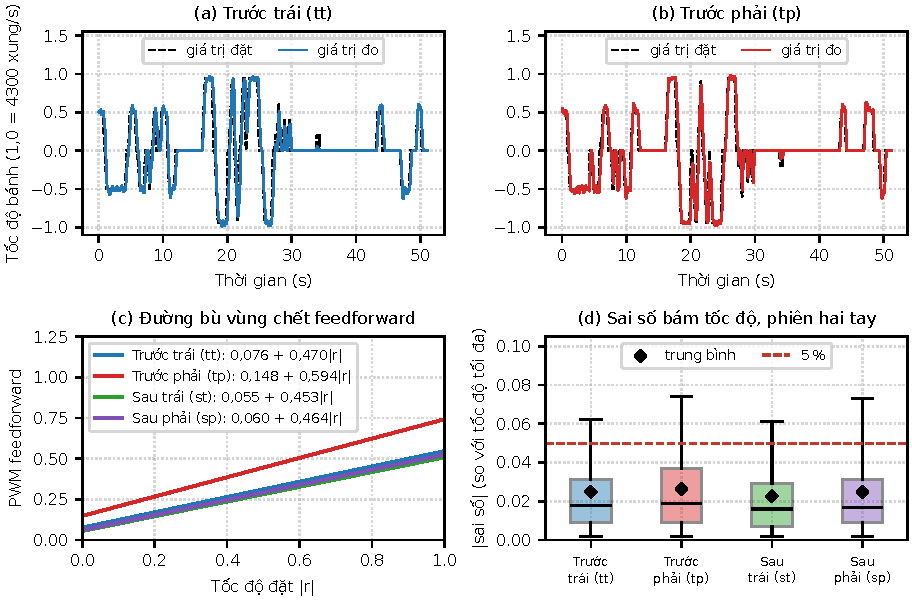
\includegraphics[width=\textwidth]{fig_wheel_vi.pdf}
  \caption{Điều khiển tốc độ bánh, phiên hai tay. (a), (b): giá trị đặt và đo của hai bánh trong 50 s; (c): đường feedforward; (d): phân bố sai số xác lập (râu: phân vị 5--95; hình thoi: trung bình; nét đứt: 5\,\%).}
  \label{fig:wheel}
\end{figure}

\textbf{Chuyển động thân robot.} Bảng~\ref{tab:odo} so lệnh với vận tốc tính từ encoder theo (\ref{eq:fk}); Hình~\ref{fig:rtt} vẽ phân bố RTT và độ lớn vận tốc. Sai lệch theo trục chính dưới 0,6\,\% khi tịnh tiến và 2,4--2,5\,\% khi xoay, chuyển động ngoài ý muốn ở các trục khác không quá 0,004. Đây là vận tốc suy ra từ encoder, chưa tính trượt bánh trên sàn nên không phải sai số vị trí thật.

\begin{table}[H]
\caption{Lệnh so với động học thuận. Sáu hàng đầu từ phiên cử chỉ v1, hai hàng chéo từ phiên v2.}
\label{tab:odo}
\centering\footnotesize\setlength{\tabcolsep}{3pt}
\begin{tabular}{lrccrr}
\toprule
Chuyển động & Mẫu & Lệnh $(v_x,v_y,\omega)$ & Từ encoder & Lệch chính & Trục khác \\
\midrule
Tiến & 543 & (+0,472; 0; 0) & (+0,474; +0,001; +0,002) & +0,6\,\% & 0,002 \\
Lùi & 360 & (-0,510; 0; 0) & (-0,510; -0,001; -0,001) & -0,1\,\% & 0,001 \\
Sang trái & 96 & (0; +0,480; 0) & (+0,004; +0,482; +0,002) & +0,4\,\% & 0,004 \\
Sang phải & 73 & (0; -0,480; 0) & (-0,003; -0,479; 0) & -0,2\,\% & 0,003 \\
Xoay trái & 238 & (0; 0; +0,435) & (+0,003; +0,001; +0,446) & +2,5\,\% & 0,003 \\
Xoay phải & 230 & (0; 0; -0,442) & (-0,001; 0; -0,453) & +2,4\,\% & 0,001 \\
Chéo tiến trái (v2) & 98 & (+0,308; +0,245; 0) & (+0,316; +0,256; +0,001) & -- & -- \\
Chéo tiến phải (v2) & 71 & (+0,313; -0,237; 0) & (+0,316; -0,243; -0,002) & -- & -- \\
\bottomrule
\end{tabular}
\end{table}

\begin{figure}[H]
  \centering
  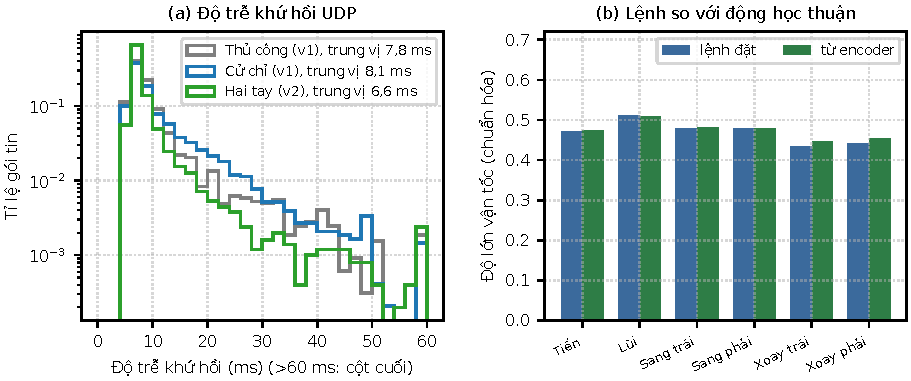
\includegraphics[width=\textwidth]{fig_rtt_odo_vi.pdf}
  \caption{(a) Phân bố RTT của ba phiên (thang log, giá trị trên 60 ms gom vào cột cuối). (b) Độ lớn vận tốc lệnh và vận tốc từ encoder cho sáu chuyển động cơ bản.}
  \label{fig:rtt}
\end{figure}

%====================================================================
\section{Giới hạn và cách tái lập}
\textbf{Giới hạn.} Số liệu từ một robot, một sàn nhà, một người vận hành. Chưa có khảo sát người dùng. Số đo con trỏ trên tay thật (rung, lệch khi click) chỉ từ một người và 12 lần click, chưa đo tỉ lệ bấm trúng; cơ chế neo FREEZE\_BACK không cho kết quả tốt hơn trong các lần đo này. Chưa có so sánh bộ điều khiển với PID thuần hay vòng hở. Chưa đo độ trễ từ camera đến bánh xe. Robot không có cảm biến vật cản.

\textbf{Tái lập số liệu và hình.} Từ thư mục gốc dự án:
\begin{center}\small
\code{.venv/bin/python reports/make\_figures.py}\quad (sinh hình và \code{reports/figures/stats.json})\\
\code{python tests/analyze\_drive\_log.py docs/data/v2/drive\_twohand.csv}\\
\code{python tests/test\_hands\_logic.py}\quad \code{python tests/camera\_fps\_test.py}
\end{center}
\end{document}
